\chapter{Scyther}
\label{chp:scyther} 

%Introduction to Scyther. What it is. How it works. Examples.

There exists multiple state-of-the-art tools for performing formal analysis of security protocols, for example Avispa \cite{avispa}, ProVerif \cite{proverif} and Scyther \cite{scyther}. This thesis uses Scyther as the tool for conducting the formal security analysis, and the following chapter will give an introduction to Scyther, how it works, and examples of usages.


\section{The Scyther Tool: Verification, Falsification, and Analysis of Security Protocols}

Scyther is a tool for both verification, falsification, and analysis of security protocols developed by Cas Cremers. The tool is based on a patter refinement algorithm that enables unbounded verification, falsification and characterization \cite{cremers2008scyther}. Scyther allows its users to verify security protocols in two different ways. The first option is to execute Scyther scripts through the command-line interface, which provides a pdf-file containing the results of protocol verification. Option two, is to use Scyther's own \gls{gui}, which provides panels for both verification results, and in case of attacks being found; a visual graph of Scyther's proposed attack on the protocol. The most recent release of Scyther was published on April 4, 2014, and is currently available for both Windows, OS X and Linux.


Scyther performs its analyses under the \emph{perfect cryptography assumption} \cite{cremers2008unbounded}. This assumption states that all cryptographic functions are perfectly designed, hence it is impossible for the adversary to learn anything about the encrypted message without possessing the corresponding decryption key.


A security protocol's specification describes messages that are sent between parties and computation done at either party's side. This can be seen as the blueprint of what the different entities are actually allowed to do, and how  

% Write(short and easy) about the algorithm.

\subsection{Scyther and its Pattern Refinement Algorithm / its novelty?}

Most algorithms used in verification tools performs \emph{bounded} verification, which means that they are capable of handling a finite space of protocol behaviours. This is a restriction, implying that the algorithm is not able to verify all possible behaviours (or states) of the protocol, but rather a finite subset of the possible state-space. One of Scyther's unique features is its ability to handle an \emph{unbounded} (or infinite) state-space, and that it is guaranteed to \emph{terminate} \cite{cremers2008unbounded}. By constructing an algorithm that terminates every time, it allows for providing useful results, even when no attack is found, or if the algorithm is not able to verify the protocol in the unbounded state-space \cite{cremers2008scyther}.

Scyther utilizes formal models for describing protocol behaviour. As these are symbolic, they are 



As mentioned, a protocol specification contains a set of roles which serves as blueprints that describes what the protocol is able to do. An execution of the protocol is referred to as a \emph{run}, and defines an unique instance of the protocol with respect to local constraints and the binding between the role and the actual agent acting out the roles behaviour. 

Other novel features implemented in Scyther includes assisted protocol analysis by providing the analyst with different classes of protocol behaviours (or attacks), as well as so-called multi-protocol analysis which allows for analysing multiple protocols that coexist in the environment.


% Bedre dette

In the event of Scyther finding an attack on the modelled protocol, Scyther will also provide proves for the attack and present a graphical view of its proposed attack.

Provides formal proofs of the security protocol in question. If Scyther finds a possible attack, it will also prove it.



For analysis of protocol security, Scyther provides different classes of attacks, which deflects from other available analysis tools.





\subsection{Reasons for Choosing Scyther}

"Scyther is chosen because of reasons."

Another reason for choosing Scyther is that it is a teaching tool, and comes with a manual and a set of exercises for aiding the user in understanding the tool and its functionality.

Move this to the end of chapter?

\section{Scyther's Different Modes of Usage}

\subsection{Verifying Claims}

When modelling security protocols in Scyther, an important part is to state security claims for each of the different parties (or \emph{roles}) of the protocol. Examples on such claims are that the key used for encryption between two roles is supposed to be secret, or that the communicating roles have authenticated each other correctly during the protocol execution. 
\begin{verbatim}
claim(Alice, Secret, AliceSecretKey);
\end{verbatim}

\subsection{Generating Claims Automatically}

If we were to develop a security protocol and not knowing the proper claims that should go with it, Scyther is able to automatically analyse our protocol and generate the appropriate claims. Scyther does so by claiming that all locally generated values and variables (such as cryptographic nonces) are supposed to be secret, before verifying them as described in the previous section.

\subsection{Complete Characterization}


In addition to verifying claims described in a protocol, Scyther is also able to present a finite set of traces that represent all the execution paths of the protocol. This information can be used to gain insight in potential problems and weaknesses of the modelled protocol. For most protocols, the set of such traces are limited to 1-5 paths, making it fairly easy to quickly obtain an oversight of the protocol's behaviour \cite{cremers2008scyther}.




\section{Claims}



\subsection{Alive}

\subsection{Secret}




\subsection{Non-injective Synchronization}

Synchronization requires that all protocol messages occur in the expected order with expected values, and that the behaviour is equivalent to as if the protocol was executed without the presence of any adversary. An injective synchronization property states that the protocol executes as expected over \emph{multiple} runs, claiming that it is not possible for an attacker to use information from previous runs into disrupting the current protocol execution \cite{cremers2005operational}. Such an attack is known as a replay attack, and is used by an adversary to inject traffic into the protocol execution to induce undesirable or unexpected behaviour.

Scyther, however, does not support this enhanced form of synchronization, hence it is vulnerable to replay attacks \cite{cremers2008scyther}. Using its language, we can claim that a property holds non-injective synchronization by using the \texttt{ni-synch} statement.


%Synchronization = Strong form for authentication. Does not protect against replay attacks. Same for Non-injective synchronization.



\subsection{Non-injective Agreement}

(weak agreement)


\subsection{Running, Commit}





 
\section{Scyther Syntax}


The syntax used in \verb!.spdl!-files, which are protocol files that can be run and verified by Scyther, can resemble popular object-oriented languages such as C, C++ or Java. The structure of a minimum working example is shown below, consisting of an outer class defining the protocol and multiple agents (or roles) inside the protocol. In this example, we define that our protocol consists of two communicating parties; Alice and Bob, without giving them any specific behaviour.

\begin{lstlisting}
protocol MinimumWorkingExampleProtocol(Alice, Bob){
	role Alice { };
	role Bob { };  
};
\end{lstlisting}


For each of the different roles in the protocol, behaviour can be added as a sequence of send and receive events, as well as variable declarations, constants and claims. For our Alice role, we can define a simple behaviour as shown below, where Alice generates a random nonce \texttt{Na} and sends it to Bob, before receiving a message from Bob containing the random nonce \texttt{Nb}. All events are labelled with either \texttt{send} or \texttt{recv} followed by a subscript and a number. The number indicates the message's position in a \gls{msc}, and must be incremented for each message. Typically, a \texttt{send}-event has a corresponding \texttt{recv}-event at the receiving role with the same number.


\begin{lstlisting}
role Alice{
	fresh Na: Nonce; # A freshly generated nonce
	var Nb: Nonce; # A variable for receiving a nonce
	
	send_1(Alice, Bob, Na); # Message sent from Alice to Bob containing Na
	recv_2(Bob, Alice, Nb); # Message sent from Bob to Alice containing Nb, which is stored as a variable
};
\end{lstlisting}


Along with support for creating fresh nonce, variables and terms, Scyther also provides a wide set of cryptographic elements such as hash functions, symmetric-key cryptography, public-key cryptography, as well as declaring user specific types and macros, which are abbreviations of complex expressions into simpler once. A sequence of events within a role are in most cases concluded with a set of claim events. Claim events are, as previous mentioned, used for describing the security properties of the role. For our Alice, we want to claim that the two nonces \texttt{Na} and \texttt{Nb} are meant to be kept secret from an adversary.


\begin{lstlisting}
role Alice{
	[...]
	
	# Claims:
	claim(Alice, Secret, Na);
	claim(Alice, Secret, Nb);
};
\end{lstlisting}


Probably elaborate more on the Scyther syntax? More examples? 

\section{Scyther's Graphical Interface for Verification and Falsification}

When running Scyther in its three modes, different views are provided through Scyther's \gls{gui}. If we continue on our example from the section on Scyther's syntax, we now want to verify the security claims for Alice's role in the protocol.

Pictures. How nice.

\begin{figure}
	\centering
	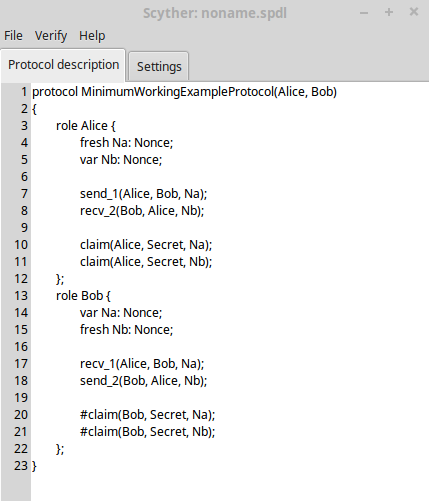
\includegraphics[scale=0.85]{ScytherMainWindow.png}
	\caption{Main view of Scyther's \gls{gui} with a window for writing scripts.}
	\label{fig:scythermain}
\end{figure}

\begin{figure}
	\centering
	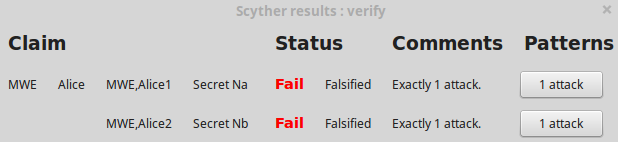
\includegraphics[scale=0.80]{ScytherVerifyFail.png}
	\caption{Main view of Scyther's \gls{gui} with a window for writing scripts.}
	\label{fig:scytherverifyfail}
\end{figure}

\begin{figure}
	\centering
	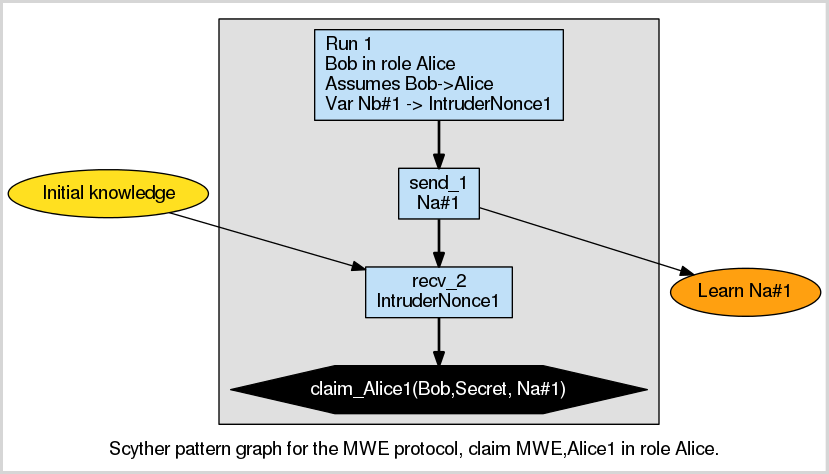
\includegraphics[scale=0.58]{ScytherFailAttackGraph.png}
	\caption{Main view of Scyther's \gls{gui} with a window for writing scripts.}
	\label{fig:scytherfailgraph}
\end{figure}

\begin{figure}
	\centering
	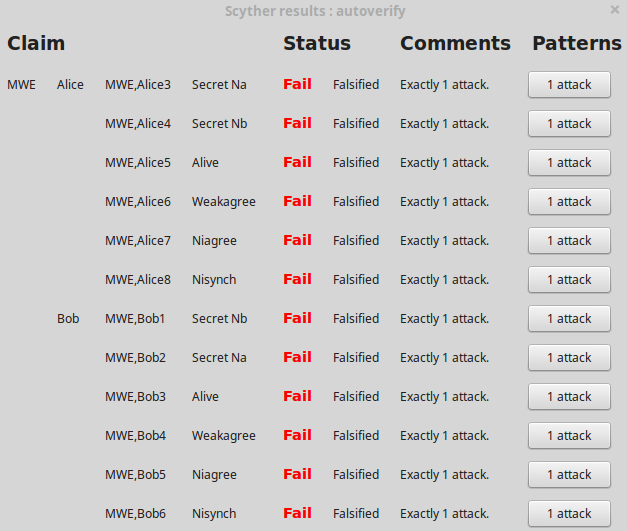
\includegraphics[scale=0.80]{ScytherAutomaticVerifyClaimsFail.png}
	\caption{Main view of Scyther's \gls{gui} with a window for writing scripts.}
	\label{fig:scytherautomaticclaims}
\end{figure}

\begin{figure}
	\centering
	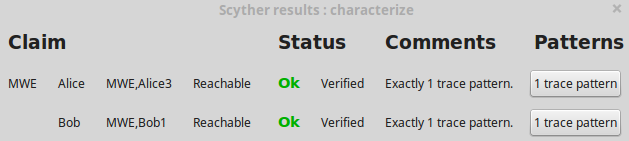
\includegraphics[scale=0.80]{ScytherCharacterizeOk.png}
	\caption{Main view of Scyther's \gls{gui} with a window for writing scripts.}
	\label{fig:scythercharacterize}
\end{figure}